\documentclass{article}
\usepackage{pgfplots}
\usepackage{amsmath}

\begin{document}

\begin{figure}[h]
    \centering
    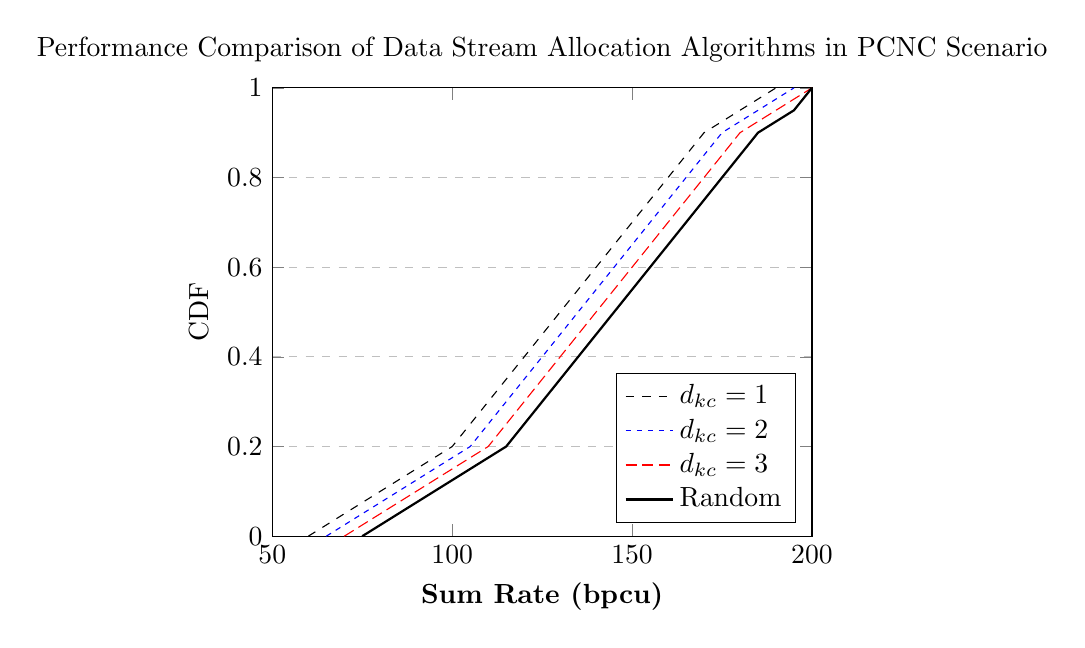
\begin{tikzpicture}
        \begin{axis}[
            xlabel={\textbf{Sum Rate (bpcu)}},
            ylabel={CDF},
            xmin=50, xmax=200,
            ymin=0, ymax=1,
            xtick={50, 100, 150, 200},
            ymajorgrids=true,
            grid style=dashed,
            legend pos=south east,
            title={Performance Comparison of Data Stream Allocation Algorithms in PCNC Scenario},
            legend cell align={left},
            legend entries={$d_{kc}=1$, $d_{kc}=2$, $d_{kc}=3$, Random, Proposed},
            ]
            
            % Dashed black line
            \addplot[dashed, black] coordinates {
                (60, 0) (70, 0.05) (80, 0.1) (90, 0.15) (100, 0.2) 
                (110, 0.3) (120, 0.4) (130, 0.5) (140, 0.6) (150, 0.7)
                (160, 0.8) (170, 0.9) (180, 0.95) (190, 1)
            };
            
            % Blue dashed line
            \addplot[dash pattern = on 2pt off 2pt, blue] coordinates {
                (65, 0) (75, 0.05) (85, 0.1) (95, 0.15) (105, 0.2) 
                (115, 0.3) (125, 0.4) (135, 0.5) (145, 0.6) (155, 0.7)
                (165, 0.8) (175, 0.9) (185, 0.95) (195, 1)
            };
            
            % Red dashed line
            \addplot[dash pattern = on 4pt off 2pt, red] coordinates {
                (70, 0) (80, 0.05) (90, 0.1) (100, 0.15) (110, 0.2) 
                (120, 0.3) (130, 0.4) (140, 0.5) (150, 0.6) (160, 0.7)
                (170, 0.8) (180, 0.9) (190, 0.95) (200, 1)
            };
            
            % Black solid line
            \addplot[solid, thick, black] coordinates {
                (75, 0) (85, 0.05) (95, 0.1) (105, 0.15) (115, 0.2) 
                (125, 0.3) (135, 0.4) (145, 0.5) (155, 0.6) (165, 0.7)
                (175, 0.8) (185, 0.9) (195, 0.95) (200, 1)
            };
        \end{axis}
    \end{tikzpicture}
    
    \caption{Performance comparison of different data stream allocation algorithms under a \gls{pcnc} scenario. Parameters: $L=10$, $M=3$, $K=10$, $N=4$, and $D=200$ m.}
    \label{fig:performance_comparison}
\end{figure}

\end{document}